\documentclass[10pt]{beamer}
\usepackage{beamerthemeshadow}
\usepackage{graphicx}
\usepackage{color}
\usepackage[utf8]{inputenc}
\usepackage{hyperref}
\usepackage{makecell}               

\usepackage[english, serbian]{babel}        

\definecolor{}{rgb}{0.5, 0.3, 0.6}
\setbeamercolor{structure}{}

\title{Tehničko i naučno pisanje}
\subtitle{-- Roboti kao nastavnici --}
\author{Jovan Mijajlović, Miona Sretenović,\\ Mina Protić, Mihailo Marković}
\institute{Matematički fakultet\\Univerzitet u Beogradu}
\date{
	\footnotesize{Beograd, 2022.}	
}

\begin{document}
\begin{frame}
	\thispagestyle{empty}
	\titlepage
\end{frame}

\addtocounter{framenumber}{-1}

\begin{frame}[fragile]\frametitle{Sadržaj}
	\tableofcontents[]
\end{frame}

\section{Roboti kao nastavnici}

\subsection{Implementacija tehnologije u nastavi}

\begin{frame}[fragile]\frametitle{Implementacija tehnologije u nastavi}
	\begin{itemize}
	\item Razvoj tehnologije i njen uticaj
	\item Potreba za digitalnim opismenjavanjem
    \item Uvođenje onlajn nastave
    \item Informatika kao obavezan predmet
	\end{itemize}
\end{frame}

\subsection{Nastavnici}

\begin{frame}[fragile]\frametitle{Nastavnici - uloga i značaj u nastavi}
	\begin{itemize}	
        \item Uloga nastavnika
        \item Entuzijazam
        \item Komunikacija i rad
        \item Šta se očekuje od nastavnika?
        \begin{figure}[h!]
        \centering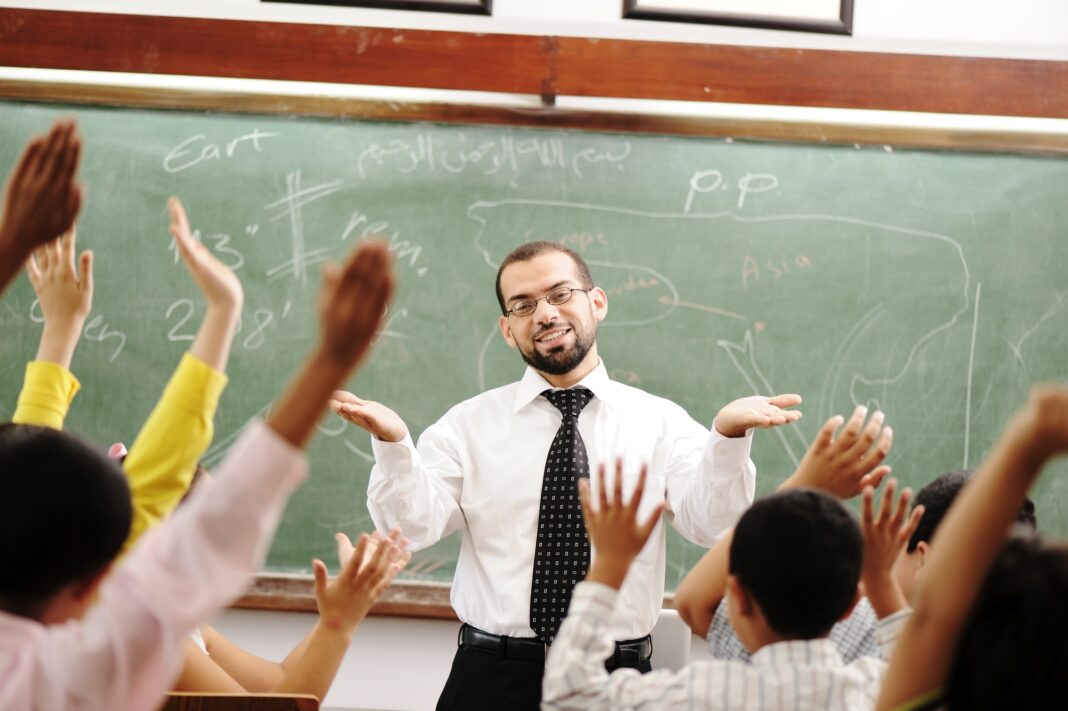
\includegraphics[height=3cm]{nastavnik.jpg} 
        \caption{Nastavnik}
        \label{fig:nastavnik}
        \end{figure}
 \end{itemize}
\end{frame}

\subsection{Roboti}
\begin{frame}[fragile]\frametitle{Roboti}
	\begin{itemize}	
        \item Šta je robot?
        \item Kako robot razmišlja?
        \item Vrste robota
    \end{itemize}

    \begin{figure}[h!]
        \centering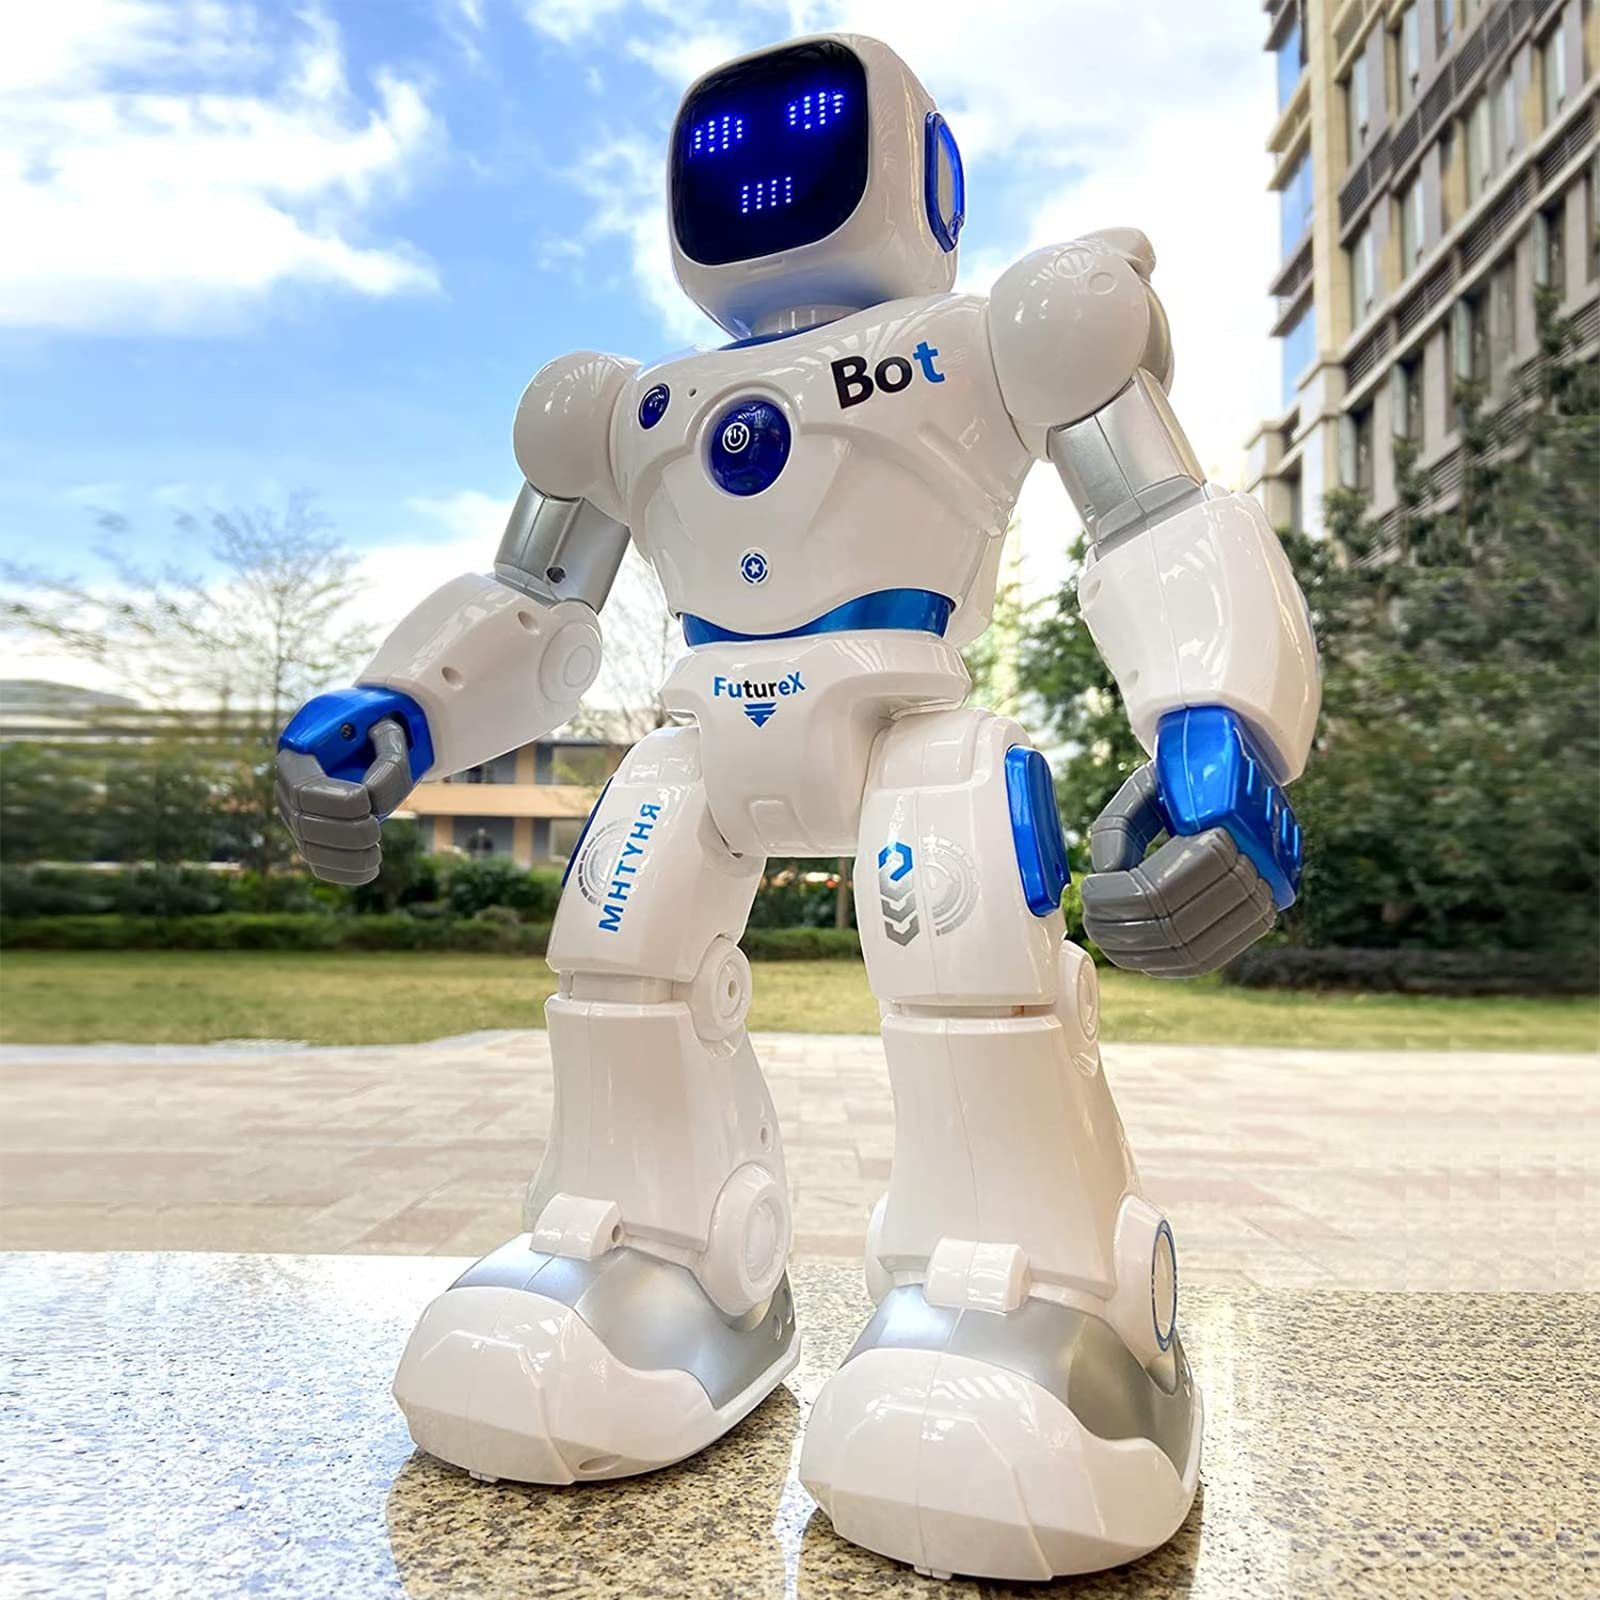
\includegraphics[height=3cm]{robot1.jpg} 
        \caption{Robot}
        \label{fig:robot}
        \end{figure}

\end{frame}

\end{document}
